%  LaTeX support: latex@mdpi.com 
%  For support, please attach all files needed for compiling as well as the log file, and specify your operating system, LaTeX version, and LaTeX editor.

%=================================================================
\documentclass[entropy,article,submit,pdftex,oneauthor]{Definitions/mdpi} 
%\documentclass[preprints,article,submit,pdftex,moreauthors]{Definitions/mdpi} 
% For posting an early version of this manuscript as a preprint, you may use "preprints" as the journal. Changing "submit" to "accept" before posting will remove line numbers.

% Below journals will use APA reference format:
% admsci, behavsci, businesses, econometrics, economies, education, ejihpe, games, humans, ijfs, journalmedia, jrfm, languages, psycholint, publications, tourismhosp, youth

% Below journals will use Chicago reference format:
% arts, genealogy, histories, humanities, jintelligence, laws, literature, religions, risks, socsci

%--------------------
% Class Options:
%--------------------
%----------
% journal
%----------
% Choose between the following MDPI journals:
% accountaudit, acoustics, actuators, addictions, adhesives, admsci, adolescents, aerobiology, aerospace, agriculture, agriengineering, agrochemicals, agronomy, ai, air, algorithms, allergies, alloys, amh, analytica, analytics, anatomia, anesthres, animals, antibiotics, antibodies, antioxidants, applbiosci, appliedchem, appliedmath, appliedphys, applmech, applmicrobiol, applnano, applsci, aquacj, architecture, arm, arthropoda, arts, asc, asi, astronomy, atmosphere, atoms, audiolres, automation, axioms, bacteria, batteries, bdcc, behavsci, beverages, biochem, bioengineering, biologics, biology, biomass, biomechanics, biomed, biomedicines, biomedinformatics, biomimetics, biomolecules, biophysica, biosensors, biosphere, biotech, birds, blockchains, bloods, blsf, brainsci, breath, buildings, businesses, cancers, carbon, cardiogenetics, catalysts, cells, ceramics, challenges, chemengineering, chemistry, chemosensors, chemproc, children, chips, cimb, civileng, cleantechnol, climate, clinbioenerg, clinpract, clockssleep, cmd, cmtr, coasts, coatings, colloids, colorants, commodities, complications, compounds, computation, computers, condensedmatter, conservation, constrmater, cosmetics, covid, crops, cryo, cryptography, crystals, csmf, ctn, curroncol, cyber, dairy, data, ddc, dentistry, dermato, dermatopathology, designs, devices, diabetology, diagnostics, dietetics, digital, disabilities, diseases, diversity, dna, drones, dynamics, earth, ebj, ecm, ecologies, econometrics, economies, education, eesp, ejihpe, electricity, electrochem, electronicmat, electronics, encyclopedia, endocrines, energies, eng, engproc, ent, entomology, entropy, environments, epidemiologia, epigenomes, esa, est, famsci, fermentation, fibers, fintech, fire, fishes, fluids, foods, forecasting, forensicsci, forests, fossstud, foundations, fractalfract, fuels, future, futureinternet, futureparasites, futurepharmacol, futurephys, futuretransp, galaxies, games, gases, gastroent, gastrointestdisord, gastronomy, gels, genealogy, genes, geographies, geohazards, geomatics, geometry, geosciences, geotechnics, geriatrics, glacies, grasses, greenhealth, gucdd, hardware, hazardousmatters, healthcare, hearts, hemato, hematolrep, heritage, higheredu, highthroughput, histories, horticulturae, hospitals, humanities, humans, hydrobiology, hydrogen, hydrology, hygiene, idr, iic, ijerph, ijfs, ijgi, ijmd, ijms, ijns, ijpb, ijt, ijtm, ijtpp, ime, immuno, informatics, information, infrastructures, inorganics, insects, instruments, inventions, iot, j, jal, jcdd, jcm, jcp, jcs, jcto, jdad, jdb, jeta, jfb, jfmk, jimaging, jintelligence, jlpea, jmahp, jmmp, jmms, jmp, jmse, jne, jnt, jof, joitmc, joma, jop, jor, journalmedia, jox, jpbi, jpm, jrfm, jsan, jtaer, jvd, jzbg, kidney, kidneydial, kinasesphosphatases, knowledge, labmed, laboratories, land, languages, laws, life, lights, limnolrev, lipidology, liquids, literature, livers, logics, logistics, lubricants, lymphatics, machines, macromol, magnetism, magnetochemistry, make, marinedrugs, materials, materproc, mathematics, mca, measurements, medicina, medicines, medsci, membranes, merits, metabolites, metals, meteorology, methane, metrics, metrology, micro, microarrays, microbiolres, microelectronics, micromachines, microorganisms, microplastics, microwave, minerals, mining, mmphys, modelling, molbank, molecules, mps, msf, mti, multimedia, muscles, nanoenergyadv, nanomanufacturing, nanomaterials, ncrna, ndt, network, neuroglia, neurolint, neurosci, nitrogen, notspecified, nri, nursrep, nutraceuticals, nutrients, obesities, oceans, ohbm, onco, oncopathology, optics, oral, organics, organoids, osteology, oxygen, parasites, parasitologia, particles, pathogens, pathophysiology, pediatrrep, pets, pharmaceuticals, pharmaceutics, pharmacoepidemiology, pharmacy, philosophies, photochem, photonics, phycology, physchem, physics, physiologia, plants, plasma, platforms, pollutants, polymers, polysaccharides, populations, poultry, powders, preprints, proceedings, processes, prosthesis, proteomes, psf, psych, psychiatryint, psychoactives, psycholint, publications, purification, quantumrep, quaternary, qubs, radiation, reactions, realestate, receptors, recycling, regeneration, religions, remotesensing, reports, reprodmed, resources, rheumato, risks, robotics, rsee, ruminants, safety, sci, scipharm, sclerosis, seeds, sensors, separations, sexes, signals, sinusitis, siuj, skins, smartcities, sna, societies, socsci, software, soilsystems, solar, solids, spectroscj, sports, standards, stats, std, stresses, surfaces, surgeries, suschem, sustainability, symmetry, synbio, systems, tae, targets, taxonomy, technologies, telecom, test, textiles, thalassrep, therapeutics, thermo, timespace, tomography, tourismhosp, toxics, toxins, transplantology, transportation, traumacare, traumas, tropicalmed, universe, urbansci, uro, vaccines, vehicles, venereology, vetsci, vibration, virtualworlds, viruses, vision, waste, water, wem, wevj, wild, wind, women, world, youth, zoonoticdis

%---------
% article
%---------
% The default type of manuscript is "article", but can be replaced by: 
% abstract, addendum, article, benchmark, book, bookreview, briefcommunication, briefreport, casereport, changes, clinicopathologicalchallenge, comment, commentary, communication, conceptpaper, conferenceproceedings, correction, conferencereport, creative, datadescriptor, discussion, entry, expressionofconcern, extendedabstract, editorial, essay, erratum, fieldguide, hypothesis, interestingimages, letter, meetingreport, monograph, newbookreceived, obituary, opinion, proceedingpaper, projectreport, reply, retraction, review, perspective, protocol, shortnote, studyprotocol, supfile, systematicreview, technicalnote, viewpoint, guidelines, registeredreport, tutorial,  giantsinurology, urologyaroundtheworld
% supfile = supplementary materials

%----------
% submit
%----------
% The class option "submit" will be changed to "accept" by the Editorial Office when the paper is accepted. This will only make changes to the frontpage (e.g., the logo of the journal will get visible), the headings, and the copyright information. Also, line numbering will be removed. Journal info and pagination for accepted papers will also be assigned by the Editorial Office.

%------------------
% moreauthors
%------------------
% If there is only one author the class option oneauthor should be used. Otherwise use the class option moreauthors.

%---------
% pdftex
%---------
% The option pdftex is for use with pdfLaTeX. Remove "pdftex" for (1) compiling with LaTeX & dvi2pdf (if eps figures are used) or for (2) compiling with XeLaTeX.

%=================================================================
% MDPI internal commands - do not modify
\firstpage{1} 
\makeatletter 
\setcounter{page}{\@firstpage} 
\makeatother
\pubvolume{1}
\issuenum{1}
\articlenumber{0}
\pubyear{2025}
\copyrightyear{2025}
%\externaleditor{Firstname Lastname} % More than 1 editor, please add `` and '' before the last editor name
\datereceived{ } 
\daterevised{ } % Comment out if no revised date
\dateaccepted{ } 
\datepublished{ } 
%\datecorrected{} % For corrected papers: "Corrected: XXX" date in the original paper.
%\dateretracted{} % For retracted papers: "Retracted: XXX" date in the original paper.
\hreflink{https://doi.org/} % If needed use \linebreak
%\doinum{}
%\pdfoutput=1 % Uncommented for upload to arXiv.org
%\CorrStatement{yes}  % For updates
%\longauthorlist{yes} % For many authors that exceed the left citation part

%=================================================================
% Add packages and commands here. The following packages are loaded in our class file: fontenc, inputenc, calc, indentfirst, fancyhdr, graphicx, epstopdf, lastpage, ifthen, float, amsmath, amssymb, lineno, setspace, enumitem, mathpazo, booktabs, titlesec, etoolbox, tabto, xcolor, colortbl, soul, multirow, microtype, tikz, totcount, changepage, attrib, upgreek, array, tabularx, pbox, ragged2e, tocloft, marginnote, marginfix, enotez, amsthm, natbib, hyperref, cleveref, scrextend, url, geometry, newfloat, caption, draftwatermark, seqsplit
% cleveref: load \crefname definitions after \begin{document}

%=================================================================
% Please use the following mathematics environments: Theorem, Lemma, Corollary, Proposition, Characterization, Property, Problem, Example, ExamplesandDefinitions, Hypothesis, Remark, Definition, Notation, Assumption
%% For proofs, please use the proof environment (the amsthm package is loaded by the MDPI class).

%=================================================================
% Full title of the paper (Capitalized)
\Title{Dynamic Assembly Theory and Information Evolution}

% MDPI internal command: Title for citation in the left column
\TitleCitation{Dynamic Assembly Theory and Information Evolution}

% Author Orchid ID: enter ID or remove command
\newcommand{\orcidauthorA}{0009-0007-7122-0317} % Add \orcidA{} behind the author's name

% Authors, for the paper (add full first names)
\Author{Dan Adler $^{1,\dagger,\ddagger}$\orcidA{}}

%\longauthorlist{no}

% MDPI internal command: Authors, for metadata in PDF
\AuthorNames{Dan Adler}

% MDPI internal command: Authors, for citation in the left column, only choose below one of them according to the journal style
% If this is a APA style journal 
% (admsci, behavsci, businesses, econometrics, economies, education, ejihpe, games, humans, ijfs, journalmedia, jrfm, languages, psycholint, publications, tourismhosp, youth): 
% Lastname, F., Lastname, F., \& Lastname, F.

% If this is a Chicago style journal 
% (arts, genealogy, histories, humanities, jintelligence, laws, literature, religions, risks, socsci): 
% Lastname, Firstname, Firstname Lastname, and Firstname Lastname.

% If this is a ACS style journal (Except for the above Chicago and APA journals, all others are in the ACS format): 
% Lastname, F.; Lastname, F.; Lastname, F.
\isAPAStyle{%
       \AuthorCitation{Adler, D.}
         }{%
        \isChicagoStyle{%
        \AuthorCitation{Adler, Dan.}
        }{
        \AuthorCitation{Adler, D.}
        }
}

% Affiliations / Addresses (Add [1] after \address if there is only one affiliation.)
\address{%
$^{1}$ \quad dan@danadler.com.com}

%\simplesumm{} % Simple summary

%\conference{} % An extended version of a conference paper

% Abstract (Do not insert blank lines, i.e. \\) 
\abstract{This paper explores the principles of dynamic assembly and information evolution by integrating insights from Assembly Theory and extending them through a forward-looking framework, ABC systems. ABC systems model the generation and persistence of patterns through probabilistic interactions and stability-driven selection, providing a versatile mechanism for understanding emergent complexity without relying on specific physical laws. The framework operates on two interdependent distributions: the population distribution, which represents the relative abundance of patterns, and the stability distribution, which governs the likelihood of successful interactions and persistence. By applying dynamic graph representations, Bayesian updating, and Lagrangian principles, this study reveals how stability gradients and resource flows lead to emergent phenomena such as catalytic cycles, adaptive pathways, and self-organization. The approach is contrasted with traditional backward-tracing methodologies in Assembly Theory, emphasizing the forward construction of novel patterns and their dependence on dynamic constraints. Through theoretical analysis and simulations, this work underscores the potential of dynamic assembly systems to model evolutionary processes, prebiotic chemistry, and the emergence of order in complex networks, providing a foundation for future research in both natural and artificial systems.}


% Keywords
\keyword{Dynamic Assembly; Information Evolution; Assembly Theory; Stability-driven Selection; Emergent Complexity; Evolutionary Dynamics; Probabilistic Interactions; Top-down and Bottom-up Causality; Information Dynamics; Roulette Wheel Selection}

% The fields PACS, MSC, and JEL may be left empty or commented out if not applicable
%\PACS{J0101}
%\MSC{}
%\JEL{}

%%%%%%%%%%%%%%%%%%%%%%%%%%%%%%%%%%%%%%%%%%
% Only for the journal Diversity
%\LSID{\url{http://}}

%%%%%%%%%%%%%%%%%%%%%%%%%%%%%%%%%%%%%%%%%%
% Only for the journal Applied Sciences
%\featuredapplication{Authors are encouraged to provide a concise description of the specific application or a potential application of the work. This section is not mandatory.}
%%%%%%%%%%%%%%%%%%%%%%%%%%%%%%%%%%%%%%%%%%

%%%%%%%%%%%%%%%%%%%%%%%%%%%%%%%%%%%%%%%%%%
% Only for the journal Data
%\dataset{DOI number or link to the deposited data set if the data set is published separately. If the data set shall be published as a supplement to this paper, this field will be filled by the journal editors. In this case, please submit the data set as a supplement.}
%\datasetlicense{License under which the data set is made available (CC0, CC-BY, CC-BY-SA, CC-BY-NC, etc.)}

%%%%%%%%%%%%%%%%%%%%%%%%%%%%%%%%%%%%%%%%%%
% Only for the journal Toxins
%\keycontribution{The breakthroughs or highlights of the manuscript. Authors can write one or two sentences to describe the most important part of the paper.}

%%%%%%%%%%%%%%%%%%%%%%%%%%%%%%%%%%%%%%%%%%
% Only for the journal Encyclopedia
%\encyclopediadef{For entry manuscripts only: please provide a brief overview of the entry title instead of an abstract.}

%%%%%%%%%%%%%%%%%%%%%%%%%%%%%%%%%%%%%%%%%%
% Only for the journal Advances in Respiratory Medicine and Smart Cities
%\addhighlights{yes}
%\renewcommand{\addhighlights}{%

%\noindent This is an obligatory section in “Advances in Respiratory Medicine'' and ``Smart Cities”, whose goal is to increase the discoverability and readability of the article via search engines and other scholars. Highlights should not be a copy of the abstract, but a simple text allowing the reader to quickly and simplified find out what the article is about and what can be cited from it. Each of these parts should be devoted up to 2~bullet points.\vspace{3pt}\\
%\textbf{What are the main findings?}
% \begin{itemize}[labelsep=2.5mm,topsep=-3pt]
% \item First bullet.
% \item Second bullet.
% \end{itemize}\vspace{3pt}
%\textbf{What is the implication of the main finding?}
% \begin{itemize}[labelsep=2.5mm,topsep=-3pt]
% \item First bullet.
% \item Second bullet.
% \end{itemize}
%}

%%%%%%%%%%%%%%%%%%%%%%%%%%%%%%%%%%%%%%%%%%
\begin{document}

%%%%%%%%%%%%%%%%%%%%%%%%%%%%%%%%%%%%%%%%%%
\section{Introduction and Background}

The emergence of complexity and information from randomness is a profound question spanning physics, biology, chemistry, and computation. Recent developments, such as Lloyd's quantum computational perspective \cite{lloyd2006programming}, Davies' exploration of information's role in biological processes \cite{davies2019demon}, Tegmark's "Mathematical Universe" \cite{tegmark2008mathematical}, and Wolfram's cellular-automata universe framework \cite{wolfram2020fundamental}, conceptualize complexity and information as emergent properties. However, these works leave unresolved how such properties arise dynamically from abiotic processes.

Assembly Theory (AT) \cite{walker2023nature} provides a powerful framework for understanding how selection shapes the generation and proliferation of complex objects by quantifying their assembly index, defined as the minimal number of recursive steps required to construct an object. By incorporating both historical contingency and selection, AT offers insights into the combinatorial explosion of possibilities in assembly spaces, illustrating how selection restricts this space to produce high-complexity objects found in abundance. However, AT typically operates from an observed object backward, constructing assembly pathways to infer the history of its formation.

This paper introduces ABC systems \cite{adler2024howinfoevolves}, which extend and complement AT by focusing on forward dynamics: modeling how patterns evolve step by step from base elements through probabilistic interactions and stability-driven selection. Unlike the retrospective approach of AT, ABC systems explore the generative processes that lead to the creation and proliferation of complex patterns in a dynamic environment. Stability constraints play a central role, as they bias interactions toward configurations that persist longer and interact more frequently, introducing an element of selection akin to that described in AT. This dynamic process has the potential to encode logical operations, computational rules, and, under certain conditions, self-replicating behaviors. The forward-building approach of ABC systems offers a practical framework for exploring the emergence of complexity, particularly in prebiotic or synthetic contexts.

By drawing connections between ABC systems and AT, this work highlights both overlapping and complementary aspects of the two frameworks. While AT provides a rigorous empirical measure of selection and assembly, ABC systems offer a predictive and generative model for understanding how stability and interaction rules shape the evolution of complexity over successive generations. This perspective bridges gaps between backward-looking and forward-building approaches to complexity, laying the groundwork for a unified theory of assembly and information evolution.

However, significant challenges remain in applying these principles to realistic prebiotic or computational models. This paper addresses these challenges by deriving theoretical insights, employing simulations, and relating the dynamics of ABC systems to established concepts from physics, chemistry, and information theory.


\subsection{Definition of ABC Systems}

We define "ABC Systems" as a population of base elements \( A, B, C, \dots \) that can form compounds through local pairwise interactions governed by unspecified forces. These elements may exist in either the physical universe or within an abstract conceptual framework. The stability of compounds determines how many generations they persist, whereas the base elements regenerate in each generation. Over successive generations, the system experiences a form of natural selection, where compound stability shapes the evolution of the population.

ABC systems evolve based on two interrelated probability distributions: the population distribution, which captures the relative abundance of patterns within the system, and the stability distribution, which reflects the likelihood of interactions yielding new and stable compounds. These distributions collectively govern the system's dynamics, driving the selection and evolution of stable patterns over generations and determining the emergent information encoded in the system.

Stability quantifies the inherent resilience of a compound against decay or dissociation. This resilience determines the lifespan of the compound. High-stability compounds persist for multiple generations, increasing their abundance and therefore their opportunities to interact and form new compounds. The stability of compounds may depend on various factors, such as energy barriers, geometric compatibility, or abstract interaction rules, making it a universal parameter applicable to diverse systems. Using an analogy to physical systems, stability can be expressed as a function of three key factors: longevity, interactivity, and environmental conditions. These factors may combine multiplicatively to yield the overall stability of a given interaction:

\[
S(p, q) = Longevity \cdot Interactivity \cdot Environment.
\]

Longevity quantifies the duration for which a pattern remains viable, increasing its likelihood of participating in future interactions. For example, the stability of \( \text{H}_2\text{O} \) molecules arises from strong covalent bonds that allow them to persist and engage in subsequent reactions. Interactivity represents the ability of a pattern to form new connections, analogous to chemical valency. Carbon, for example, exhibits high valence, enabling the formation of a vast array of stable compounds. Environmental conditions, such as temperature, pressure, and concentration, govern the likelihood of patterns forming or persisting. Ice formation, for instance, depends critically on both temperature and pressure, while higher concentrations of reactants promote productive interactions.

The dynamic evolution of ABC systems is driven by a fixed replenishment of base elements, ensuring a consistent influx of resources that sustain interaction and pattern formation. This replenishment prevents stagnation and allows the system to explore a wide range of configurations over successive generations. As interactions occur, stable compounds accumulate, leading to the emergence of complex patterns and feedback loops that reinforce their persistence.

This framework bears similarities to Assembly Theory (AT), which also quantifies the generation of complexity through recursive processes. In AT, the assembly index measures the minimum number of recursive steps needed to construct an object, and selection is inferred from observing high-complexity objects in abundance. Unlike AT, which primarily works backward from observed objects to infer assembly pathways, ABC systems take a forward-looking approach, modeling the generative processes that lead to complexity. In this way, ABC systems emphasize the role of probabilistic interactions and stability-driven selection in real-time evolution.

By integrating concepts from AT, ABC systems provide a complementary perspective, focusing on how stability influences the exploration of assembly spaces and the dynamic interplay between top-down and bottom-up causality. A previous paper \cite{adler2024howinfoevolves} highlights several key emergent phenomena of ABC systems, such as entropy reduction, and the dynamic interplay between these causal structures. Through simulations and theoretical analysis, it shows how ABC systems can encode information, compute logic, and generate self-organizing behaviors without invoking external design or intelligent agents. The forward-building approach of ABC systems offers a novel perspective for understanding complexity in natural and synthetic systems.

\subsection{Connections to Assembly Theory and Distinct Contributions}

Assembly Theory (AT) \cite{walker2023nature} provides a framework for understanding the emergence of complexity by tracing the assembly pathways of observed objects. AT quantifies an object’s complexity through its assembly index, which measures the minimum number of steps required to construct it from elementary building blocks. This backward-tracing approach emphasizes historical contingency, revealing the combinatorial explosion of possibilities and the selective processes that constrain observed outcomes. Concepts such as the assembly universe (AU), assembly possible (AP), and assembly contingent (AC) delineate the combinatorial, physically feasible, and historically influenced spaces, respectively.

ABC systems, by contrast, adopt a forward-looking perspective, modeling the generative process of evolving patterns through probabilistic interactions and stability-driven selection. Starting with base elements ($A$, $B$, $C$), ABC systems simulate iterative interactions and stability-guided evolution, highlighting the mechanisms by which certain configurations persist and proliferate. This forward approach complements AT by focusing on the dynamic processes that generate complexity rather than reconstructing it from observed structures.

Both frameworks explore how selection shapes the combinatorial space of possibilities. While AT employs the assembly index to infer selection retrospectively, ABC systems dynamically encode selection via stability constraints, which influence the persistence and interactions of patterns in real-time. Unlike AT’s static definitions, the context-dependency of stability in ABC systems reflects the impact of environmental factors such as temperature, pressure, and resource availability, offering a more dynamic and adaptable model.

ABC systems also extend AT’s forward dynamics by explicitly modeling resource replenishment, turnover, and feedback loops. These features allow for the exploration of how stability gradients and environmental constraints shape complexity in evolving systems. In this way, ABC systems provide a complementary lens to AT, enriching our understanding of the interplay between historical contingency and dynamic evolution.

The integration of AT’s historical focus and ABC systems’ dynamic perspective reveals new insights into the evolution of complexity. AT excels at quantifying the cumulative effects of selection and historical pathways, while ABC systems emphasize the processes of pattern discovery and stabilization. Together, these approaches highlight selection as a unifying principle, whether inferred retrospectively or modeled prospectively, and provide a framework for understanding the emergence of complexity across natural and artificial systems.

By bridging these perspectives, this work extends the applicability of evolutionary principles, offering insights into phenomena ranging from prebiotic chemistry to complex networks. ABC systems, with their focus on stability-driven dynamics, complement AT’s focus on assembly indices and contingent spaces, contributing to a unified understanding of how order and information arise in diverse contexts.



\section{Unrestricted vs ABC Systems: Expected distributions}

The dynamics of an unrestricted system and ABC systems diverge fundamentally in the distribution of compounds formed over successive generations. This difference arises from the constraints imposed on ABC interactions, leading to different statistical behaviors in the two systems.

\subsection{Unrestricted Systems}

Unrestricted systems allow all pairwise interactions between elements and compounds, leading to a combinatorial explosion of the state space. At each generation, new compounds are formed uniformly, without biases or constraints. The probability of observing a compound \( p \) at generation \( t \) is given by:
\begin{equation}
P(p_t) = \frac{1}{N},
\end{equation}
where \( N \) is the total number of compounds. As \( t \) increases, \( N \) grows combinatorially, causing \( P(p_t) \to 0 \), reflecting the uniform dispersion of probabilities across an expanding state space. This results in a highly diffuse distribution where no compound dominates.

\subsection{ABC Systems}

In contrast, an ABC system introduces stability constraints that guide the evolution of the state space. Compounds are no longer produced with equal likelihood; instead, their formation and persistence are influenced by their abundance, stability, interactions, and flows within the system. These constraints create a self-reinforcing feedback loop, where stable compounds dominate token flows and new compounds emerge through probabilistically weighted interactions.

Unlike the unrestricted system, the expected distribution of compounds in an ABC system cannot be predicted analytically for the system's long-term behavior. The state space evolves dynamically, shaped by both the probabilistic creation of new compounds and the preferential allocation of base elements to high-stability compounds. Let \( P(p_t) \) denote the probability of observing compound \( p \) at generation \( t \) in the ABC system. The distribution is governed by:
\begin{equation}
P(p_{t+1}) \propto P(p_t) \cdot \sum_{q \in P} P(q_t) \cdot S(p, q),
\end{equation}
where \( S(p, q) \) represents the stability of the interaction between \( p \) and \( q \). This equation reflects the evolutionary nature of the system, where the probability of a compound in generation \( t+1 \) depends on its prior probability and the stability-weighted flows into it. 

\subsection{Implications of the Distributional Differences}

The uniformity of the unrestricted system reflects its ergodic exploration of an unbounded state space. No single compound is likely to dominate, and the system does not exhibit any adaptive evolution. In contrast, the ABC system evolves nonuniformly, with high-stability compounds emerging as attractors for flows, leading to self-reinforcing pathways and punctuated equilibrium \cite{gould1977punctuated} dynamics. Unlike the unrestricted system, where entropy increases, the entropy of an ABC system may decrease due to stability selection.

These contrasting behaviors highlight the importance of stability and constraints in guiding the evolution of complex systems. The uniform distribution of the unrestricted system shows its inability to sustain or prioritize specific patterns, while the ABC system demonstrates how selection pressures can induce emergent structures and adaptive behaviors. In subsequent sections, we will explore how Bayesian updating and stability-driven flows further shape the evolution of ABC systems.

\section{Simulation Framework and Results}

To compare the dynamics of unrestricted and ABC systems, we developed a simulation framework that models the evolution of token flows and compound formation over successive generations. This framework captures the key differences between the two systems: the uniform expansion of the state space in the unrestricted system and the stability-driven selection pressures in the ABC system. The simulation results provide quantitative information on the distribution of patterns, their evolution, and the role of stability constraints.

\subsection{Simulation Framework}

The simulation begins with an initial population of base elements and evolves over a fixed number of generations. In each generation, tokens interact to form new compounds, which are added to the population. The rules governing these interactions differ between the unrestricted and ABC systems.

For the \textbf{unrestricted system}, interactions between all elements and compounds are allowed. This results in a combinatorial expansion of the state space, with new compounds formed uniformly and without preference for stability. The simulation does not enforce constraints, allowing the system to explore its full potential state space.

For the \textbf{ABC system}, interactions are influenced by stability constraints. Each compound is assigned a stability weight and the interactions are probabilistically weighted by these values. Higher-stability compounds attract more tokens, reinforcing their dominance in the token flow and shaping the evolution of the state space. In addition, token flows are compacted into more readable forms, ensuring the interpretability of the simulation results. The simulation can be described with the following pseudocode:

\scriptsize
\begin{center}
\begin{minipage}{0.7\textwidth}
\ttfamily
\begin{verbatim}
Initialize population with base elements (e.g., A, B, C)
For each generation:
    Remove expired elements
    Replenish base elements
    Randomly select pairs of elements to interact and form new compounds
    For each interaction:
        If Unrestricted System:
            Form compound and add to population
        If ABC System:
            Weight interactions by stability
            Add formed compound to population
    Compact patterns into simplified representations
    Store population data for analysis
\end{verbatim}
\end{minipage}
\end{center}
\normalsize

The differences between ABC systems and unrestricted elements occur in two places: ABC elements expire because they have lifetimes determined by their stability, and the random selection of pairs in ABC systems implicitly implements roulette wheel selection \cite{goldberg1989genetic} \cite{holland1975adaptation} because there are more instances of stable elements over time. 

\subsection{Simulation Results}

The results of the simulation reveal stark contrasts between the unrestricted and ABC systems. In the unrestricted system, the state space expands combinatorially, producing a uniform distribution of compounds. As the number of generations increases, the probability of observing any specific compound diminishes to near zero as a result of the unbounded growth of the state space. This uniformity reflects the ergodic nature of the system, with tokens evenly distributed across all possible compounds.

In the ABC system, by contrast, stability constraints induce a highly skewed distribution of compounds. High-stability patterns act as attractors, drawing token flows and concentrating the population in specific pathways. The feedback loop created by stability weighting ensures that stable compounds persist over generations, while less stable patterns diminish in importance.

Figure \ref{fig:simulation_results} illustrates these differences. The unrestricted system exhibits a broad and diffuse distribution of tokens with no dominant patterns. However, the ABC system shows pronounced concentrations in high-stability compounds, with clear pathways emerging over successive generations.

\begin{figure}[h]
    \centering
    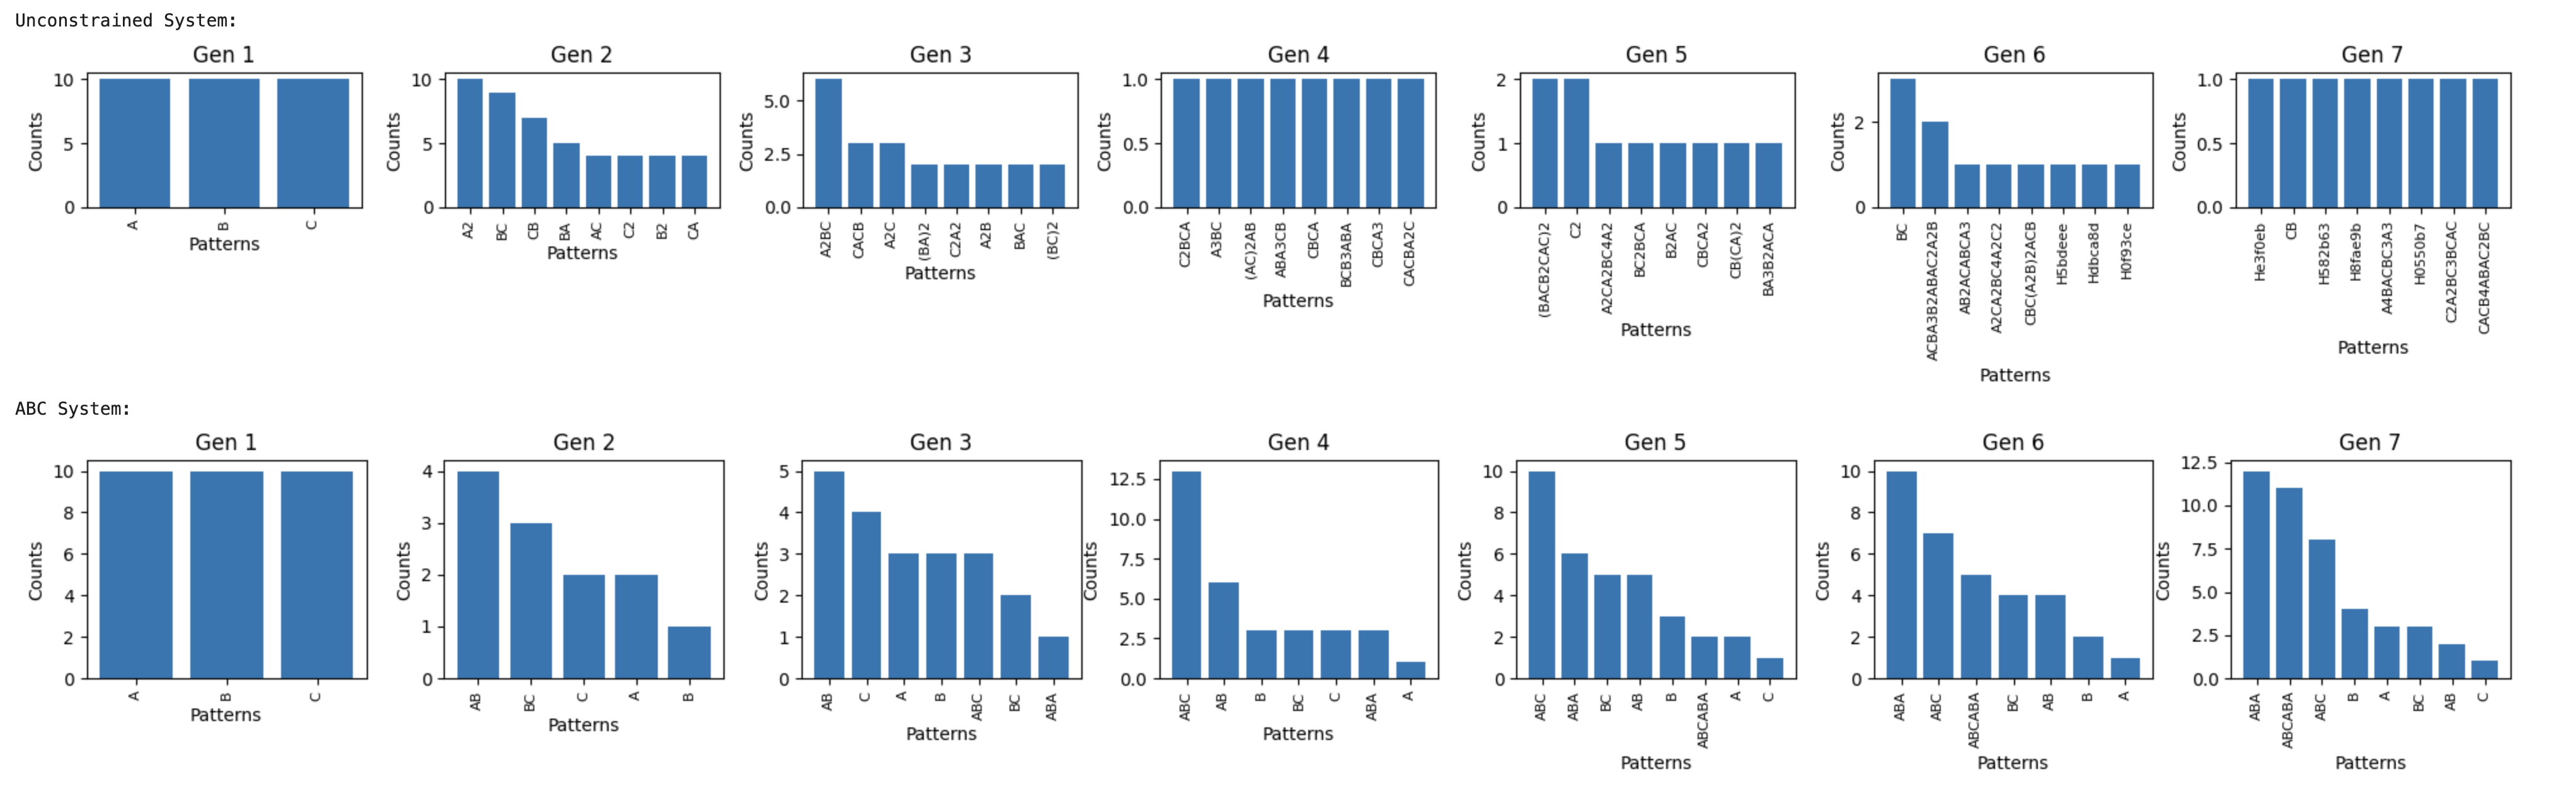
\includegraphics[width=1\textwidth,height=7cm]{monte-carlo-fits.png}
    \caption{Comparison of the evolution of the unrestricted system and the ABC system. The unrestricted system demonstrates a uniform distribution across an expanding state space, while the ABC system concentrates tokens in high-stability patterns, leading to emergent pathways.}
    \label{fig:simulation_results}
\end{figure}

The unrestricted system exemplifies the behavior of an unconstrained probability space, where the combinatorial explosion of possibilities ensures that no single compound dominates. Its entropy approaches the maximum value.

In contrast, the ABC system highlights the impact of stability constraints on evolving systems. Stability-weighted interactions drive the emergence of dominant patterns, reducing entropy, and creating pathways of concentrated token flows. The simulation results provide a foundation for further analysis of stability-driven dynamics and their implications, as explored in subsequent sections of this paper.

\section{Bayesian Updating in ABC and the Unconstrained Systems}

ABC systems highlight a key distinction between Bayesian \cite{mcgrayne2011theory} updating and frequentist probabilities, illustrating their respective roles in evolving versus static systems. Bayesian updating provides a dynamic framework for incorporating information between generations, making it a hallmark of systems capable of evolution and self-organization. In this context, the "prior" has a literal meaning, referring directly to the probability distribution of the prior generation, rather than a subjective interpretation of probability or a framework for hypothesis testing.

This interpretation reflects the dependency between the probability distributions in successive generations in any evolving system. Specifically, in ABC systems, the evolving state space emerges from the interactions and stabilities of patterns, leading to a probability space that changes over time. At any specific generation, the probabilities are frequentist, describing the relative frequencies of patterns. However, the evolution of these probabilities across generations is inherently Bayesian, since the prior distribution directly influences the current generation.

\subsection{Bayesian Updating in ABC Systems}

In ABC systems, the probability of a pattern \( p \) in generation \( t+1 \) depends on its prior probability \( P(p_t) \), the probabilities of other patterns \( P(q_t) \), and the stability of their interactions \( S(p, q) \):

\begin{equation}
P(p_{t+1}) = \frac{P(p_t) \cdot \sum_{q \in P} P(q_t) \cdot S(p, q)}{\sum_{p' \in P} P(p'_t) \cdot \sum_{q \in P} P(q_t) \cdot S(p', q)}
\label{eq:bayes}
\end{equation}

where \( P(p_t) \) is the prior probability of p in generation t, \( P(q_t) \) is the probability of interacting patterns q in generation t, and \( S(p, q) \) is the stability of interactions that produce or sustain p through q. This formula can be directly related to Bayes' theorem by realizing that \( P(p_{t+1}) \) is conditionally dependent on the set of observed patterns \( O_t \) generated in the prior generation. Using Bayes' theorem:
\begin{equation}
P(p_{t+1}) = P(p_t | O_t) = \frac{P(O_t | p_t) \cdot P(p_t)}{P(O_t)},
\end{equation}
where:
\begin{enumerate}
    \item[] \( P(p_t) \): The prior probability of \( p \) in generation \( t \), representing its abundance in the previous generation.
    \item[] \( P(O_t | p_t) \): The likelihood that \( p \) contributes to the generation of the observed interactions \( O_t \), determined by the stabilities \( S(p, q) \).
    \item[] \( P(O_t) \): The normalization term, summing over all patterns \( p' \):
    \[
    P(O_t) = \sum_{p' \in P} P(O_t | p'_t) \cdot P(p'_t).
    \]
\end{enumerate}

This relationship captures the evolving nature of the probability space, where the observed interactions \( O_t \) act as a feedback mechanism that biases the distribution towards patterns that are more stable or frequent. In contrast, unconstrained systems lack such feedback, as stability is uniform and all patterns interact equally, resulting in a uniform probability distribution that does not evolve over generations. 

This interpretation emphasizes the dual role of Bayes' formula in ABC systems, as generational memory, where the prior \( P(p_t) \) ensures continuity by preserving information about patterns from the previous generation.
It also serves as selective amplification, where likelihood \( P(O_t | p_t) \) introduces selection pressure by favoring patterns that contribute more to observed interactions. 

Traditionally viewed as a tool for updating subjective beliefs based on new information, Bayes’ theorem in the context of ABC systems highlights its role in linking successive generations through probabilistic interactions and stability constraints. This generational link underscores the applicability of the theorem to evolving systems, where the "prior" is literally the distribution of the prior generation of the system \cite{le2020equation}.

\subsection{Bayesian vs Markov Analysis in Evolutionary Systems}

The Bayesian framework described above provides a basis for comparing ABC systems with Markov analysis. Although ABC systems exhibit generational dependency akin to a Markov process, they differ fundamentally due to their dynamically expanding state space, nonstationary transition probabilities, and the evolutionary significance of individual pathways rather than global distributions. 

In a classical Markov process \cite{norris1997markov}, the probability of transitioning to a new state depends only on the current state, expressed as \( P(O_{t+1} \mid O_t) \). For ABC systems, this dependency is captured by the Bayesian update rule derived earlier in Eq.~(\ref{eq:bayes}). If we attempt to frame ABC systems in a Markovian context, we consider the joint probability of all patterns in \( O_{t+1} \) given \( O_t \). This would be expressed as:
\begin{equation}
P(O_{t+1} \mid O_t) = \prod_{p \in O_{t+1}} P(p_{t+1}),
\end{equation}
where \( P(p_{t+1}) \) is derived from the Bayesian update formula. However, this joint probability approach aligns poorly with the typical ABC system analysis goals, since it aggregates over all possible evolutionary pathways without distinguishing the specific transitions that drive the system dynamics.

Markov-based tools, such as transition matrices or joint probability distributions, are less suited to analyzing ABC systems because of several limitations inherent to the Markovian framework. In classical Markov chains, the state space is fixed, allowing for a static transition matrix. In ABC systems, the state space expands dynamically as new patterns emerge, making it infeasible to pre-define or maintain a complete transition matrix. Markov processes often assume stationary transition probabilities that remain constant over time. In ABC systems, transition probabilities evolve with each generation, driven by stability constraints, interactions, and the emergence of new patterns. This nonstationarity requires recalculating transition probabilities at every step, undermining the utility of standard Markov tools.

Hidden Markov models (HMMs) \cite{rabiner1989hmm} also do not appear very promising, as they model systems where hidden states drive the observable dynamics, and these hidden states are key to uncovering latent structures. In ABC systems, the core mechanisms, such as stabilities, token flows, and probabilistic interactions, are already explicitly modeled, which makes the HMM framework somewhat redundant.

ABC system analysis typically prioritizes the specific evolutionary pathways the system takes, tracing the formation and persistence of individual patterns. The Bayesian formula directly addresses this by updating the probability of each pattern based on prior abundances, interactions, and stability. In contrast, Markov approaches aggregate the joint probability distribution of all patterns, obscuring the details of specific transitions. Stability values in ABC systems bias interactions, introducing selection pressure that amplifies certain patterns over others. Although Markov chains can represent biases through weighted transitions, they do not naturally account for the feedback mechanisms and adaptive dynamics encoded in the Bayesian framework.

ABC systems are designed to model the exploration of new possibilities, where interactions produce novel patterns that were not part of the prior generation. Markov processes are ill-suited for this type of open-ended generativity, as they rely on a predefined set of states and transitions.

The Bayesian framework overcomes these limitations by focusing on the probabilities of individual patterns and their generational updates. The Bayesian formula in Eq.~(\ref{eq:bayes}) directly captures the dynamics of pattern evolution, integrating prior probabilities, interaction dynamics, and stability constraints. This generational update aligns with the goals of ABC systems, enabling the analysis of specific pathways and their adaptive significance. By focusing on individual patterns rather than the joint distribution, the Bayesian approach provides a clearer view of how selection pressure and stability drive the emergence of dominant patterns. This focus on pathways, coupled with the ability to model evolving state spaces and nonstationary dynamics, makes the Bayesian framework a more natural and insightful tool for analyzing ABC systems.

\subsection{Exploring Mass Action Kinetics in the Context of ABC Systems}

Mass Action Kinetics (MAK) \cite{TuranyiTomlin2014} provides a well-established framework in chemistry to describe the evolution of reactant concentrations over time through deterministic rate equations. The principles of MAK, rooted in stoichiometry and reaction rates, are particularly effective for modeling systems with predefined reactions and a fixed set of chemical species.

In MAK, the dynamics of a system are governed by rate equations of the form:
\begin{equation}
\frac{d[A]}{dt} = -k[A][B],
\end{equation}
where \( [A] \) and \( [B] \) represent the concentrations of reactants, and \( k \) is the reaction rate constant. These equations enforce strict conservation laws for mass and energy, ensuring that the total amount of reactants and products remains constant across all reactions. This conservation constraint is analogous to the way ABC systems track the counts of patterns across generations, ensuring that interactions respect stability and population dynamics.

Despite these similarities, MAK imposes a critical limitation: the set of reactions must be specified a priori. This means that MAK does not support the evolutionary discovery of new patterns or compounds, a hallmark of ABC systems. In MAK, the reactions and their rate laws are immutable, leading to a closed system that lacks the flexibility to explore novel configurations or emergent behaviors.

The deterministic framework of MAK also contrasts with the probabilistic nature of ABC systems. In MAK, reaction rates directly determine the changes in concentrations, resulting in smooth and predictable trajectories over time. ABC systems, on the contrary, operate probabilistically, with interactions guided by stability values and prior abundances. This stochasticity introduces variability and adaptability, allowing ABC systems to explore Kauffman's concept of the "adjacent possible" \cite{kauffman1996investigations} and generate unforeseen patterns through combinatorial interactions.

Although MAK does not inherently support open-ended generativity, its principles can still be adapted to certain aspects of ABC systems. For instance, MAK-style equations could be employed to approximate the dynamics of stable patterns in ABC systems, treating stability values as analogs to reaction rate constants. These equations would describe how the population of stable patterns evolves over generations, providing a deterministic view of this subset of the system.

\section{Dynamic Graph Representation and Token Flow Analysis}

To further investigate the dynamics of ABC systems, we represent the state of the system in a specific generation as a directed graph, where the nodes correspond to patterns $AB$, $ABA$, $ABC$, and the directed edges represent the interactions that occurred between them. Recall that the base elements $A$, $B$, $C$ are replenished in each generation, initiating a cascade of interactions that propagate "tokens" (shown in Figure~\ref{fig:abc_sim} as the count $N$ of instances of each pattern). The tokens accumulate at the nodes based on the flow dynamics governed by stability (shown in Figure~\ref{fig:abc_sim} as $S$).

\begin{figure}[h]
    \centering
    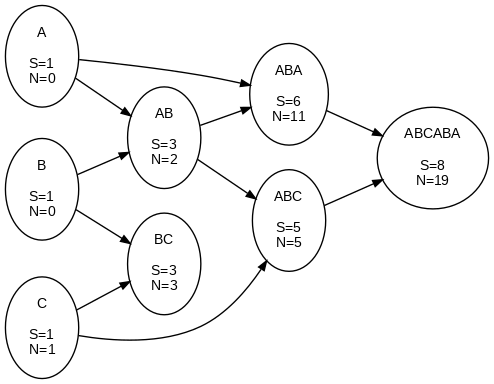
\includegraphics[width=0.5\linewidth]{abc_graph.png}
    \caption{Graph representation of an ABC system showing stability (S), and the number of instances or tokens (N) of each base element and compound.}
    \label{fig:abc_sim}
\end{figure}

The dynamic graph in Figure~\ref{fig:abc_sim} represents the 7th generation of the simulation shown in Figure~\ref{fig:simulation_results}. The distribution of tokens across the graph reveals insights into the self-reinforcing nature of stability in ABC systems. Nodes with higher stability values (\textit{e.g.}, $ABCABA$) attract more tokens, leading to the emergence of dominant patterns. This phenomenon reflects a feedback loop: As tokens accumulate at a stable node, it becomes increasingly likely to dominate subsequent interactions, establishing preferential flow paths through the graph. Consequently, the system's token traffic converges to well-defined routes, concentrating resources on a subset of high-stability patterns while marginalizing less stable ones.

However, the graph may change significantly between generations if a new disruptor node emerges in the system. A disruptor node is characterized by a high stability value and strategic positioning within the graph, enabling it to compete with previously dominant nodes for token traffic. This disruptor can reroute flows, effectively redistributing tokens and breaking established dominance patterns. 

From a physical perspective, the behavior of token flows in the ABC system parallels physical phenomena such as those observed in fluid systems, where a new high-conductivity channel can divert flow away from existing pathways. Similarly, in RC circuits, the introduction of a new low-resistance branch redistributes the current, altering the overall system equilibrium. In chemical systems, such as lattice reactions or yeast metabolic chains, stability thresholds determine which reaction pathways dominate, with external perturbations capable of reconfiguring flow patterns.

Dynamic graphs have been used for switch-level simulation of transistor networks \cite{AdlerCAD}, where graph pathways are dynamically determined by the state of the on transistors, enabling specific connections to guide current flow. Similarly, in ABC systems, token flow is governed by stability and probabilistic interactions, determining which nodes persist and propagate. Both frameworks employ dynamic graphs to model evolving pathways, where stability in ABC systems plays an analogous role to conductance, influencing the flow dynamics within each generation.

\subsection{Polymerization as an Example of ABC Systems}

To illustrate the principles of ABC systems in a real-world context, we present a polymerization reaction graph (see Figure~\ref{fig:polymerization_graph}), which models the stepwise assembly of polymer chains from ethylene (\( \text{C}_2\text{H}_4 \)) monomers. 

\begin{figure}[h!]
    \centering
    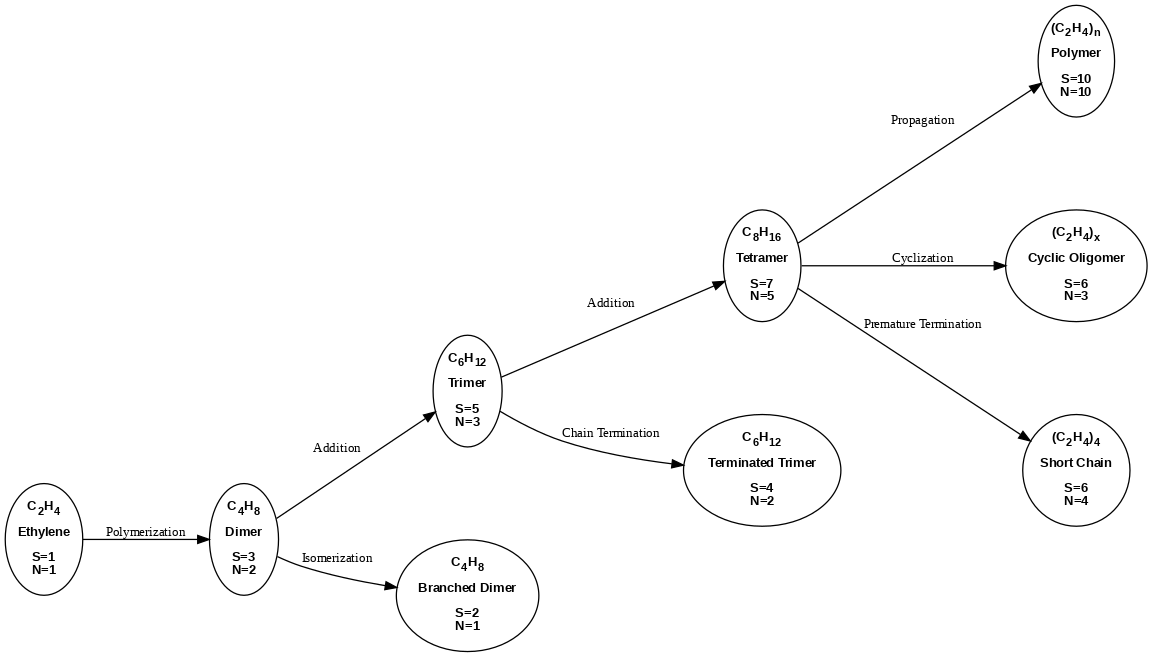
\includegraphics[width=\textwidth]{abc_poly.png}
    \caption{Polymerization reaction graph illustrating the stepwise assembly of polymer chains from ethylene (\( \text{C}_2\text{H}_4 \)) monomers. Nodes represent chemical species, annotated with their stability (\( S \)) and relative abundance (\( N \)), while edges depict possible reaction pathways. The graph highlights both stable pathways leading to linear polymers and less stable intermediates, showcasing the evolutionary dynamics of ABC systems.}
    \label{fig:polymerization_graph}
\end{figure}

This graph captures the formation of intermediate species such as dimers (\( \text{C}_4\text{H}_8 \)), trimers (\( \text{C}_6\text{H}_{12} \)), and tetramers (\( \text{C}_8\text{H}_{16} \)), eventually leading to the formation of a polymer chain. Additionally, less stable by-products such as branched dimers, terminated trimers, and cyclic oligomers are included to emphasize the evolutionary aspect of the system. Each node in the graph represents a chemical species, annotated with its stability (\( S \)) and relative abundance (\( N \)), while the edges depict possible reaction pathways.

This example is analogous to the ABC system framework as it models the flow of base elements and compounds through a network of interactions governed by stability constraints. Stability in this context reflects the thermodynamic and kinetic properties of the species: compounds with higher stabilities (e.g., the polymer) are more likely to persist and accumulate over successive reactions, while less stable species (e.g., branched or terminated intermediates) are transient or exist in lower abundances. The replenishment of ethylene monomers ensures a continuous supply of resources, akin to the base element replenishment in ABC systems.

The stabilities assigned in the polymerization graph are chosen based on the underlying chemistry. For instance, linear oligomers are generally more stable than branched or cyclic intermediates due to reduced steric strain and favorable chain interactions. The polymer exhibits the highest stability as it represents the thermodynamically favored product in the absence of termination processes. Conversely, species such as branched dimers and cyclic oligomers have lower stabilities because their formation pathways are less favorable energetically or kinetically.

This example also highlights the similarities and differences between ABC systems and Assembly Theory (AT). Both frameworks address the combinatorial explosion of possible configurations during assembly processes. In AT, the assembly index quantifies the minimal number of recursive steps required to construct an object. In the polymerization graph, this would correspond to the number of monomer additions needed to produce each species. However, ABC systems differ by emphasizing forward dynamics and the role of stability constraints in shaping evolutionary pathways. Unlike the retrospective analysis in AT, which traces observed objects back to their precursors, ABC systems focus on the probabilistic emergence of patterns and their persistence under environmental conditions. 

\section{Lagrangian Analysis of ABC Systems}

The flow dynamics of tokens in ABC systems can be elegantly captured by interpreting high-stability nodes as low-potential energy wells within the probability space. Nodes with greater stability, \( S(p) \), attract tokens, driving their accumulation and strengthening self-organized paths. This concept of "demand" naturally translates into a potential energy framework, where the potential energy of a node is inversely related to its stability. Token redistribution can also be analyzed in terms of the "effort" required for transitions between nodes. This effort is analogous to kinetic energy.

The potential energy \( U \) reflects the stability-weighted demand at each node. For a node \( p \), the contribution of potential energy depends on the stability of its incoming edges and the token counts at neighboring nodes. The potential energy of node \( p \) is given by:
\begin{equation}
U(p) = -\sum_{q \in \text{neighbors}(p)} S(p, q) \cdot N_q,
\end{equation}
where \( N_q \) is the number of tokens at neighboring node \( q \). Through replenishment, base nodes gain an additional contribution to their potential energy:
\begin{equation}
U_{\text{replenish}}(p) = -R_p \cdot S(p),
\end{equation}
where \( R_p \) is the replenishment rate for node \( p \). The total potential energy across the graph is therefore:
\begin{equation}
U = \sum_{p} \left( -\sum_{q \in \text{neighbors}(p)} S(p, q) \cdot N_q - R_p \cdot S(p) \right).
\end{equation}

The kinetic energy \( T \) quantifies the redistribution effort required for token flows between nodes. It is derived by analogy to classical mechanics, where the kinetic energy is proportional to the square of the velocity and weighted by the mass. In the ABC system, the flow rate \( \frac{\Delta N_{pq}}{\Delta t} \) replaces velocity, and the stability \( S(p, q) \) acts as an effective inertial mass, modulating the cost of redistribution based on the stability of interactions. Summing over all pairs of interacting nodes yields the total kinetic energy, with higher stability reducing the redistribution cost and higher flow rates increasing it. This formulation captures the dynamic effort to maintain token flows in the evolving system. For a flow of tokens from node \( p \) to node \( q \), the contribution to the kinetic energy is given by:
\begin{equation}
T_{pq} = \frac{1}{2} S(p, q) \left( \frac{\Delta N_{pq}}{\Delta t} \right)^2,
\end{equation}
where:
\begin{itemize}
    \item[] \( S(p, q) \) is the stability of the interaction between \( p \) and \( q \),
    \item[] \( \Delta N_{pq} \) is the number of tokens flowing from \( p \) to \( q \) in time \( \Delta t \).
\end{itemize}
Summing over all edges in the graph, the total kinetic energy is:
\begin{equation}
T = \sum_{(p, q)} \frac{1}{2} S(p, q) \left( \frac{\Delta N_{pq}}{\Delta t} \right)^2.
\end{equation}
Combining these terms, the Lagrangian \(\mathcal{L} = T - U \) becomes:
\begin{equation}
\mathcal{L} = \sum_{(p, q)} \frac{1}{2} S(p, q) \left( \frac{\Delta N_{pq}}{\Delta t} \right)^2 + \sum_{p} \left( \sum_{q \in \text{neighbors}(p)} S(p, q) \cdot N_q + R_p \cdot S(p) \right).
\label{eq:lagrange}
\end{equation}

This formulation provides a complete description of the system's dynamics, where \( T \) quantifies the redistribution effort, and \( U \) captures the stability-driven potential landscape. The evolution of the system is governed by minimizing the action \( \mathcal{A} \), which is the time integral of the Lagrangian \cite{goldstein2002classical}: 
\begin{equation}
\mathcal{A} = \int \mathcal{L} \, dt.
\label{eq:action}
\end{equation}

When we analyze some edge cases of \( \mathcal{A} \), the following dynamics emerges: For the case where all stabilities are equal \(S(p, q) = S_0\) for all \(p, q\), the kinetic term becomes uniform, and the potential energy term simplifies to an equal contribution across all nodes. This leads to a uniform distribution of token flow, as the system minimizes the action by equalizing \(\Delta N_{pq} / \Delta t\) at all edges. Consequently, no preferential redistribution occurs, and the system reflects the uniform state space dynamics of unconstrained systems.

In contrast, when one node dominates in stability (\(S(p, R) \gg S(p, q)\) for all \((p, q) \neq (p, R)\)), the potential energy term is heavily weighted towards the dominant node. The action is minimized by directing most of the token flow to this node, effectively making it a sink for the token flow. The remaining nodes receive negligible contributions, mirroring the collapse of token dynamics into a single dominant pathway.

Other edge cases highlight additional insights. For instance, when two nodes compete with comparable stabilities, the token flow splits proportionally to their relative stabilities, leading to shared dominance that reflects bifurcation dynamics. Sparse stability landscapes, where only a subset of nodes have non-zero stability, create isolated clusters of token flow, forming sparse localized networks. Dynamic stabilities, which evolve over time, drive transitions between equilibria, revealing the system's capacity for adaptation. 

\subsection{Comparison with Supply-Demand Perspective of ABC Systems}

The dynamics of token flows in ABC systems can also be interpreted through a supply-demand framework, which provides a complementary node-centric perspective. In this view, the stability distribution determines the "demand" for tokens at each node, while the token flow along edges fulfills this demand based on the available "supply."  The supply at a node \(p\) is given by:
\begin{equation}
\text{Supply}(p) = R_p + \sum_{q \in \text{neighbors}(p)} \Delta N_{qp},
\end{equation}
where \(R_p\) is the replenishment rate at node \(p\) and \(\Delta N_{qp}\) is the flow of tokens from neighboring nodes \(q\) to \(p\). Conversely, the demand at node \(p\) is proportional to the stability-weighted contributions of its neighbors:
\begin{equation}
\text{Demand}(p) = \sum_{q \in \text{neighbors}(p)} S(p, q) \cdot N_q,
\end{equation}
where \(S(p, q)\) is the stability between \(p\) and \(q\), and \(N_q\) is the token count at \(q\). At equilibrium, supply and demand balance at each node:
\begin{equation}
R_p + \sum_{q \in \text{neighbors}(p)} \Delta N_{qp} = \sum_{q \in \text{neighbors}(p)} S(p, q) \cdot N_q.
\end{equation}
This balance determines the distribution of token flows \(\Delta N_{pq}\) throughout the system. The supply-demand framework provides results consistent with the Lagrangian edge case analysis discussed earlier:
\begin{itemize}
    \item[] For uniform stabilities (\(S(p, q) = S_0\)), the flows \(\Delta N_{pq}\) are distributed uniformly, resulting in a flat supply-demand curve.
    \item[] For a dominant stability node, the flows concentrate on the dominant node, creating a sharply peaked supply-demand curve.
    \item[] For competing nodes with comparable stabilities, flows split proportionally, resulting in multiple peaks.
    \item[] For sparse stability landscapes, token flows localize around nodes with nonzero stability, producing isolated points on the curve.
\end{itemize}

This agreement underscores the complementary nature of the supply-demand and Lagrangian perspectives. The former highlights localized flow dynamics at nodes, while the latter emphasizes the global minimization of the action integral. Together, they provide a unified understanding of token redistribution in ABC systems.

\section{Punctuated Equilibrium and Disruption in ABC Systems}

The dynamics of ABC systems are not static; they are characterized by periods of equilibrium, where established flows dominate, interspersed with disruptive events that radically alter the flow landscape. This behavior parallels the concept of punctuated equilibrium, originally developed in evolutionary biology to describe long periods of stability disrupted by rapid evolutionary change. In ABC systems, this manifests itself as the sudden emergence of new nodes with high stability, capable of redirecting flows and forcing the system to adjust to a new equilibrium.

Consider the graph in Figure~\ref{fig:abc_sim} with a dominant high-stability node, such as \( ABCABA \) (stability \( S = 8 \)). If a new node \( ABCABC \) emerges with even higher stability (\( S = 10 \)), the flow to \( ABCABA \) can be diverted entirely or partially to the new node. The appearance of \( ABCABC \) would alter the flow dynamics throughout the graph, as the tokens are reallocated to optimize for the new potential landscape. This transition could trigger a cascade of secondary flow redirects as the system seeks a new equilibrium, reshaping the dominance hierarchy of patterns.

The potential for disruption arises from the unbounded nature of the state space. New nodes form probabilistically through interactions, meaning the system's evolution is inherently nondeterministic during periods of active node creation. However, during periods of equilibrium—when few if any new nodes are formed—the system's dynamics are more predictable, with flows stabilizing along established pathways. These stable periods can persist for long durations, punctuated by the stochastic emergence of highly stable disruptor nodes.

This behavior can be illustrated with an example from organic chemistry. Consider polysaccharide chains, which can be represented as long strings of \( \text{C}_x(\text{H}_2\text{O})_y \). These chains may grow to hundreds of units (\( x, y \sim 100 \)) before a more stable yeast-like structure is formed. Beyond this, growth to thousands of units (\( x, y \sim 1000 \)) may occur before cellulose emerges as a highly stable product. Such transitions are rare because the stability gradients along the growth paths only become strong after hundreds of relatively unconstrained linkages are added. The probability of reaching these long chains is low, and the system remains in a quasi-equilibrium state dominated by smaller, less stable polysaccharides. This is likely why complex polysaccharides like cellulose do not spontaneously form in nature; their formation pathways require extraordinary conditions to overcome the low-probability barrier of intermediate configurations.

\section{Conclusions and Future Directions}

This study advances the understanding of the evolution of complexity and information by expanding the framework of ABC systems, a model based on stability-driven selection and probabilistic interactions. Unlike abstract approaches such as Wolfram’s cellular computation \cite{wolfram2020fundamental} or Tegmark’s “Mathematical Universe” hypothesis \cite{tegmark2008mathematical}, ABC systems are grounded in physical realism, capturing the dynamics of emergent complexity through iterative interactions and feedback mechanisms.

The integration of insights from Assembly Theory (AT) \cite{walker2023nature} highlights the complementary yet distinct contributions of ABC systems. AT provides a powerful retrospective framework for analyzing how objects are constructed and selected in nature, using the assembly index to quantify the minimum number of steps required to assemble a given object. ABC systems, in contrast, adopt a forward-looking perspective that dynamically models the generation of patterns through resource flows, stability constraints, and probabilistic interactions. While AT focuses on reconstructing historical pathways, ABC systems emphasize the processes by which stability and environmental factors shape the evolution of complexity over successive generations. 

One significant innovation of ABC systems is the explicit incorporation of stability as a dynamic, context-dependent parameter influenced by environmental factors such as temperature, pressure, and resource availability. This allows ABC systems to model real-world constraints more directly than AT, where stability and selection are inferred from observed objects. By coupling stability-driven dynamics with forward generative processes, ABC systems offer a framework for exploring how complexity arises and evolves under realistic physical and chemical conditions.

This work also establishes theoretical connections between ABC systems and broader principles in physics, biology, and computation. The derivation of a Lagrangian formulation aligns ABC dynamics with the principle of least action, demonstrating how resource allocation and emergent phenomena are governed by stability gradients and feedback loops. These findings underscore the universality of ABC systems in modeling diverse processes, from autocatalytic cycles in biochemical systems to energy redistribution in physical networks.

The current study has practical implications for modeling chemical and biological networks, particularly when compared with the backward-looking approach of AT. For example, the polymerization example discussed in this work illustrates how ABC systems capture the iterative construction of complex molecules, incorporating both environmental constraints and stability feedback. Such forward dynamics provide a natural complement to AT’s assembly index, offering new perspectives on the interplay between selection, stability, and evolution in both natural and artificial systems.

Future research directions include generalizing ABC systems to support \( n \)-ary interactions through hypergraph representations, enabling the modeling of complex reactions and networks. Incorporating catalytic effects, dynamic stability, and temporal dynamics would enhance the realism of ABC systems, allowing for more accurate simulations of evolutionary processes. Additionally, exploring the integration of energy constraints, such as activation energy and conservation laws, could align ABC systems more closely with physical and chemical principles, extending their applicability to areas like metabolic networks, material self-assembly, and prebiotic chemistry.

In conclusion, ABC systems provide a versatile and generative framework for studying the emergence of complexity and information. By bridging the forward dynamics of ABC systems with the retrospective analysis of AT, this work contributes to a unified understanding of how selection, stability, and feedback drive the evolution of complexity across disciplines. These insights open new pathways for interdisciplinary research, with applications ranging from prebiotic evolution to synthetic biology and complex network dynamics.


\begin{adjustwidth}{-\extralength}{0cm}
%\printendnotes[custom] % Un-comment to print a list of endnotes
\reftitle{References}

% Please provide either the correct journal abbreviation (e.g. according to the “List of Title Word Abbreviations” http://www.issn.org/services/online-services/access-to-the-ltwa/) or the full name of the journal.
% Citations and References in Supplementary files are permitted provided that they also appear in the reference list here. 

\begin{thebibliography}{999}
    %1
    \bibitem{lloyd2006programming} S. Lloyd, \textit{Programming the Universe: A Quantum Computer Scientist Takes on the Cosmos} (Knopf, 2006).
    %2
    \bibitem{davies2019demon} P. Davies, \textit{The Demon in the Machine: How Hidden Webs of Information Are Solving the Mystery of Life} (University of Chicago Press, 2019).
    %3
    \bibitem{tegmark2008mathematical} M. Tegmark, "The Mathematical Universe," \textit{Foundations of Physics} \textbf{38}, 101-150 (2008).
    %4
    \bibitem{wolfram2020fundamental} S. Wolfram, \textit{A Project to Find the Fundamental Theory of Physics} (Wolfram Media, 2020).
    %4.5
    \bibitem{walker2023nature}
    S. I. Walker, L. Cronin, and others,
    "Assembly theory explains and quantifies selection and evolution across physical and biological systems,"
    \textit{Nature}, \textbf{618}, 619-628 (2023),
    doi:10.1038/s41586-023-06600-9.
    %5
    \bibitem{adler2024howinfoevolves} D. Adler, "How Information Evolves," \textit{Preprints}, 2024, \url{https://www.preprints.org/manuscript/202412.1649/v1}.
    %6
    \bibitem{landau1987fluid} L. D. Landau and E. M. Lifshitz, \textit{Fluid Mechanics}, 2nd ed. (Pergamon, 1987).
    %7
    \bibitem{mascolell1995microeconomic} A. Mas-Colell, M. D. Whinston, and J. R. Green, \textit{Microeconomic Theory} (Oxford University Press, 1995).
    %8
    \bibitem{gould1977punctuated}
    S. J. Gould and N. Eldredge, ``Punctuated equilibria: the tempo and mode of evolution reconsidered,'' Paleobiology \textbf{3}, 115–151 (1977).
    %9
    \bibitem{goldberg1989genetic}
    Goldberg, D.E. \textit{Genetic Algorithms in Search, Optimization, and Machine Learning}; Addison-Wesley: Boston, MA, USA, 1989.
    %10
    \bibitem{holland1975adaptation}
    Holland, J.H. \textit{Adaptation in Natural and Artificial Systems}; University of Michigan Press: Ann Arbor, MI, USA, 1975.
    %11
    \bibitem{mcgrayne2011theory}
    McGrayne, S.B. \textit{The Theory That Would Not Die: How Bayes' Rule Cracked the Enigma Code, Hunted Down Russian Submarines, and Emerged Triumphant from Two Centuries of Controversy}; Yale University Press: New Haven, CT, USA, 2011.
    %12
    \bibitem{le2020equation} N. Le, \textit{The Equation of Knowledge: From Bayes’ Rule to a Unified Philosophy of Science}, Philosophical Press, New York, NY, 2020.
    %13
    \bibitem{norris1997markov}
    J. R. Norris, \emph{Markov Chains}. Cambridge University Press, Cambridge, UK, 1997, ISBN: 978-0521633963.
    %14
    \bibitem{rabiner1989hmm}
    L. R. Rabiner, ``A Tutorial on Hidden Markov Models and Selected Applications in Speech Recognition,'' 
    \emph{Proceedings of the IEEE}, vol.~77, no.~2, pp.~257--286, 1989, doi:10.1109/5.18626.
    %15
    \bibitem{TuranyiTomlin2014}
    T. Turányi and A. S. Tomlin, \emph{Analysis of Kinetic Reaction Mechanisms}, Springer, Berlin, Heidelberg, 2014. DOI: \href{https://doi.org/10.1007/978-3-642-38724-0}{10.1007/978-3-642-38724-0}.
    %16
    \bibitem{kauffman1996investigations}
    S. A. Kauffman, \emph{Investigations}, (Oxford University Press, New York, 2000).
    %17
    \bibitem{AdlerCAD}
    D. Adler, ``Switch Level Simulation Using Dynamic Graph Algorithms,'' \emph{IEEE Transactions on Computer-Aided Design of Integrated Circuits and Systems}, vol.10, March 1991.
    %18
    \bibitem{goldstein2002classical} H. Goldstein, C. Poole, and J. Safko, \textit{Classical Mechanics}, 3rd ed. (Addison-Wesley, 2002).
    %19
    \bibitem{bohm1980wholeness}
    D. Bohm and B. J. Hiley, \emph{The Undivided Universe: An Ontological Interpretation of Quantum Theory}, Routledge, London, 1993. ISBN: 978-0415065887.

\end{thebibliography}

% If authors have biography, please use the format below
%\section*{Short Biography of Authors}
%\bio
%{\raisebox{-0.35cm}{\includegraphics[width=3.5cm,height=5.3cm,clip,keepaspectratio]{Definitions/author1.pdf}}}
%{\textbf{Firstname Lastname} Biography of first author}
%
%\bio
%{\raisebox{-0.35cm}{\includegraphics[width=3.5cm,height=5.3cm,clip,keepaspectratio]{Definitions/author2.jpg}}}
%{\textbf{Firstname Lastname} Biography of second author}

% For the MDPI journals use author-date citation, please follow the formatting guidelines on http://www.mdpi.com/authors/references
% To cite two works by the same author: \citeauthor{ref-journal-1a} (\citeyear{ref-journal-1a}, \citeyear{ref-journal-1b}). This produces: Whittaker (1967, 1975)
% To cite two works by the same author with specific pages: \citeauthor{ref-journal-3a} (\citeyear{ref-journal-3a}, p. 328; \citeyear{ref-journal-3b}, p.475). This produces: Wong (1999, p. 328; 2000, p. 475)

%%%%%%%%%%%%%%%%%%%%%%%%%%%%%%%%%%%%%%%%%%
%% for journal Sci
%\reviewreports{\\
%Reviewer 1 comments and authors’ response\\
%Reviewer 2 comments and authors’ response\\
%Reviewer 3 comments and authors’ response
%}
%%%%%%%%%%%%%%%%%%%%%%%%%%%%%%%%%%%%%%%%%%
\PublishersNote{}
%\isPreprints{} % If the paper is ``preprints'', please uncomment this parenthesis.
\end{document}

